
hola
\input{headers.tex}

\begin{document}

\section{Sheet 2}
\begin{enumerate}

%% EXERCISE 1
\item Show that a face $F$ of a polytope $P$ is exactly the convex hull of all vertices of $P$ contained in~$F$. 
In particular, $P$~has only finitely many faces.

By proposition 2.3, $F$ is a polytope (2.3.i) with $vert(F)=vert(P)\cap F$ (2.3.iii). By proposition 2.2, $F=conv(vert(F))=conv(vert(P)\cap F)$, so we have showed that a face $F$ of a polytope $P$ is exactly the convex hull of all vertices of $P$ contained in ~$F$.

By definition, every polytope $P$ can be written as the convex hull of a finite set of points $V$. By proposition 2.2.ii, $vert(P)\subset V$ for all possible $V$ defining $P$. Since $vert(F)\subset vert(P) \quad\forall F\subset P$ face, and every subset of $vert(P)$ determines at most 1 face, the number of possible faces is bounded by $2^{\#vert(P)}$, which is finite.

%% EXERCISE 2
\item Let $P\subset\R^d$, $Q\subset\R^e$ be two non-empty polytopes. Prove that the set of faces of the cartesian product polytope $P\times Q=\{(p,q)\in\R^{d+e}:p\in P,\; q\in Q\}$ exactly equals $\{F\times G: F\text{ is face of }P, \;G\text{ is face of }Q\}$. Conclude that
\[
    f_k(P\times Q)
    \ = \
    \sum_{%\substack{
      i+j=k,\;i,j\ge0}f_i(P) f_j(Q)
    \qquad
    \text{for } k\ge0.
\]

Let us show that $F\times G$ is a face of $P\times Q$, where $F$ and $G$ are faces of $P$ and $Q$, respectively. Write \[
\begin{array}{c}
 F=\left\{y\in\R^d:ay=b\right\}\cap P\text{, where } a\in(\R^d)^*, b\in\R \text{ and }P\subset\left\{y\in\R^d:ay\leq b\right\}\\
 G=\left\{z\in\R^e:cz=d\right\}\cap Q\text{, where } c\in(\R^e)^*, d\in\R \text{ and }Q\subset\left\{z\in\R^e:cz\leq d\right\}
\end{array}
\]

Note that \[
\begin{split}
F\times G=\left\{\left(\begin{array}{c}
                 y \\ z
                \end{array}
\right)\in\R^{d+e}:ay=b, \quad cz=d, \quad y\in P, \quad z\in Q\right\} \subset \\
\subset \left\{\left(\begin{array}{c}
                 y \\ z
                \end{array}\right)
\in\R^{d+e}:\left(\begin{array}{c}
                    a \\ c
                   \end{array}\right)^\top
                   \left(\begin{array}{c}
		      y \\ z
		  \end{array}\right)
=b+d \quad y\in P, \quad z\in Q\right\}
\end{split}\]

so $F\times G$ is a face of $P\times Q$ if, and only if, $\left(\begin{array}{c}
                    a \\ c
                   \end{array}\right)^\top
                   \left(\begin{array}{c}
		      y \\ z
		  \end{array}\right)
\leq b+d \quad \forall y\in P, z\in Q$ and the inclusion can be turned into an equality.

It is easy to see that $\left(\begin{array}{c}
                    a \\ c
                   \end{array}\right)^\top
                   \left(\begin{array}{c}
		      y \\ z
		  \end{array}\right)
\leq b+d \quad \forall y\in P, z\in Q$, since $ay\leq b \quad \forall y\in P$ and $cz\leq d \quad \forall z\in Q$ by hypothesis.

About the inclusion, a priori we cannot ensure that it is an equality, since there could exist, $y,z$ such that $ay=\tilde b, cz=\tilde d$, with $\tilde b + \tilde d = b+d$.

However, suppose $\tilde b > b$. Then we would have $y\in P$, with $ay > b$, which is a contradiction. So $\tilde b \leq b$. Analogously, $\tilde d \leq d$. Thus, $\tilde b = b$ and $\tilde d = d$, so the inclusion is actually an equality and $F\times G$ is a face of $P\times Q$.

(Falta la otra inclusión)

\[
\begin{align}
\begin{split}
  f_k(P\times Q)&=\\
  &=\#\left\{\text{faces } H\neq\varnothing \text{ of }P\times Q: dim(H)=k\right\}=\\
  &=\#\left\{\text{faces } F\times G:F\neq\varnothing \text{ face of }P, G\neq\varnothing \text{ face of }Q, dim(F)+dim(G)=k\right\}=\\
  &=\sum_{i+j=k; i,j\geq 0} \#\left\{\text{faces } F \text{ of } P : dim(F)=i\right\}
  \cdot\#\left\{\text{faces } G \text{ of } Q : dim(G)=j\right\}=\\  
  &=\sum_{i+j=k; i,j\geq 0} f_i(P)f_j(Q)
\end{split}
\end{align}
\]

%% EXERCISE 3
\item Show that all induced cycles of length $3$, $4$ and $5$ in the graph of a simple $d$-polytope~$P$ are graphs of $2$-faces of $P$.
Conclude that the Petersen graph is not the graph of any polytope of any dimension. (\emph{Hint for $5$-cycles:} First show this for $d=3$. Then prove
that any $5$-cycle in a simple polytope is contained in some $3$-face,
and use that faces of  simple polytopes are simple.)

\item Let $n\in\N$ be an integer and $S$ denote a subset of
  $\{1,2,\dots,\lfloor\frac{n}{2}\rfloor\}$.  
  The \emph{circulant graph} $\Gamma_n(S)$ is the graph whose vertex set is $\Z_n$, and whose edge set is the set of pairs of vertices whose difference lies in $S\cup (-S)$. 

The following figure collects all connected circulant graphs on up to $8$~vertices. Determine the \emph{polytopality range} for as many of these graphs as you can, i.e., the set of integers~$d$ such that the graph in question is the graph of a $d$-dimensional polytope.

% \bigskip
% 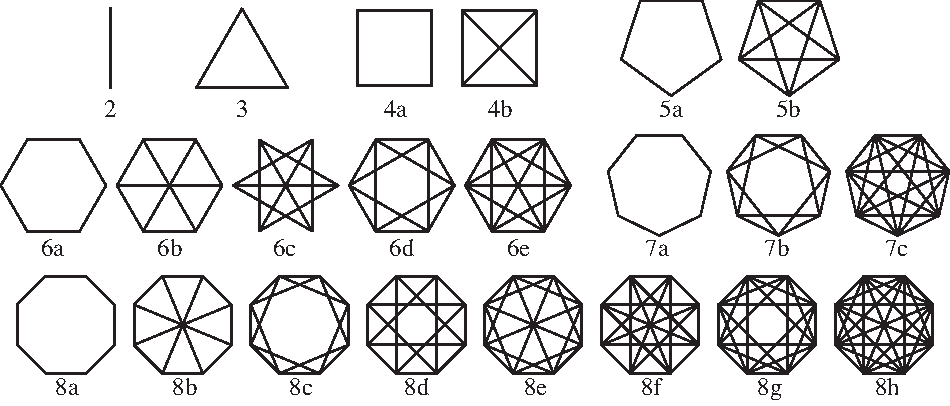
\includegraphics[width=\linewidth]{circulant}

\item Let $\Box^d$ be the $d$-dimensional $\pm1$-cube. How large can the volume of a simplex in $\Box^d$ become? (\emph{Hint:} \url{en.wikipedia.org/wiki/Hadamard_inequality}. Write a  C++ program to attain explicit bounds for $d\ge2$ as large as you can.)
\end{enumerate}

\end{document}





